\documentclass[12pt]{article}
\usepackage[margin=1in]{geometry} 
\usepackage{graphicx}
\usepackage{amsmath,amsthm,amssymb}
\usepackage{hyperref}
\usepackage{amssymb}

\title{
    \textbf{Assignment 3} \\ 
    \textbf{AI2000} \\
    \textbf{Foundations of Machine Learning}
}

\DeclareMathOperator{\E}{\mathbb{E}}

\author{
    \textbf{Darpan Gaur} \\
    \textbf{CO21BTECH11004}
}


\date{}

\begin{document}
\maketitle

\hrulefill

\section*{Problem 1}
\begin{equation*}
    E_D(w) = \frac{1}{2} \sum_{n=1}^{N} \sigma_n(y_n - w^T \phi(x_n))^2
\end{equation*}
Given dataset $D = \{(x_1, y_1), (x_2, y_2), \ldots, (x_N, y_N)\}$. 
Let $X = \begin{bmatrix} \phi(x_1) \\ \phi(x_2) \\ \vdots \\ \phi(x_N) \end{bmatrix}^T$ and $Y = \begin{bmatrix} y_1 \\ y_2 \\ \vdots \\ y_N \end{bmatrix}$, 
where $\phi(x_n)$ is the feature vector of $x_n$.
\\ \\
Error in matrix form:
\begin{equation*}
    E_D(w) = \frac{1}{2} (Y - Xw)^T \Sigma (Y - Xw)
\end{equation*}
where $\Sigma = diag(\sigma_1, \sigma_2, \ldots, \sigma_N)$, is a diagonal matrix with $\sigma_n$ on the diagonal.
\\ \\ 
Differentiating $E_D(w)$ w.r.t. $w$:
\begin{equation*}
    \frac{\partial E_D(w)}{\partial w} = \frac{1}{2} \frac{\partial}{\partial w} (Y - Xw)^T \Sigma (Y - Xw)
\end{equation*}
\\ \\
Using the property $\frac{\partial}{\partial w} x^T A x = x^T (A + A^T) \frac{\partial x}{\partial w}$, we get:
\begin{equation*}
    \frac{1}{2} \frac{\partial}{\partial w} (Y - Xw)^T \Sigma (Y - Xw) = \frac{1}{2} (Y - Xw)^T (\Sigma + \Sigma^T) \frac{\partial}{\partial w} (Y - Xw)
\end{equation*}

\begin{equation*}
    \implies
    \frac{\partial E_D(w)}{\partial w} = -(Y - Xw)^T \Sigma X
\end{equation*}

Putting $\frac{\partial E_D(w)}{\partial w} = 0$:
\begin{equation*}
    \implies
    -(Y - Xw)^T \Sigma X = 0
\end{equation*}

\begin{equation*}
    \implies
    X^T \Sigma Y = X^T \Sigma X w
\end{equation*}

\begin{equation*}
    \boxed{w = (X^T \Sigma X)^{-1} X^T \Sigma Y}
\end{equation*}

\section*{Problem 2}
\begin{equation*}
    E(w) = - \sum_{n=1}^{N} \sum_{k=1}^{K} t_{nk} log y_{k} (x_n, w) 
\end{equation*}
For a given input $x_n$, Differentiating $E(w)$ w.r.t. $a_k$:
\begin{equation*}
    \frac{\partial E(w)}{\partial a_k} = - \sum_{k=1}^{K} \frac{\partial}{\partial a_k} t_{k} log y_{k} (x_n, w) = - \sum_{k=1}^{K} \frac{\partial}{\partial y_k} t_{k} log y_{k} (x_n, w) \frac{\partial y_k}{\partial a_k} = - \sum_{k=1}^{K} \frac{t_{k}}{y_{k}} \frac{\partial y_k}{\partial a_k}
\end{equation*}

\begin{equation*}
    \frac{\partial E(w)}{\partial a_k} = - \sum_{\substack{i=1 \\ i \neq k}}^{K} \frac{t_{i}}{y_{i}} \frac{\partial y_i}{\partial a_k} - \frac{t_{k}}{y_{k}} \frac{\partial y_k}{\partial a_k}
\end{equation*}

Differentiating $y_i$ w.r.t. $a_k$:
% write 2 cases here, i = k and i != k, like piecewise function
\begin{equation*}
    \frac{\partial y_i}{\partial a_k} = \frac{\partial}{\partial a_k} \frac{e^{a_i}}{\sum_{j=1}^{K} e^{a_j}} = \frac{ - e^{a_i} e^{a_k}}{(\sum_{j=1}^{K} e^{a_j})^2} = - y_i y_k
\end{equation*}
\begin{equation*}
    \frac{\partial y_k}{\partial a_k} = \frac{\partial}{\partial a_k} \frac{e^{a_k}}{\sum_{j=1}^{K} e^{a_j}} = \frac{e^{a_k} \sum_{j=1}^{K} e^{a_j} - e^{a_k} e^{a_k}}{(\sum_{j=1}^{K} e^{a_j})^2} = y_k (1 - y_k)
\end{equation*}
Putting the values of $\frac{\partial y_i}{\partial a_k}$ and $\frac{\partial y_k}{\partial a_k}$ in $\frac{\partial E(w)}{\partial a_k}$:
\begin{equation*}
    \frac{\partial E(w)}{\partial a_k} = - \sum_{\substack{i=1 \\ i \neq k}}^{K} \frac{t_{i}}{y_{i}} (- y_i y_k) - \frac{t_{k}}{y_{k}} y_k (1 - y_k)
\end{equation*}
\begin{equation*}
    \implies
    \frac{\partial E(w)}{\partial a_k} = \sum_{\substack{i=1 \\ i \neq k}}^{K} t_{i} y_k + t_{k} y_{k} - t_{k}
\end{equation*}
\begin{equation*}
    \implies
    \frac{\partial E(w)}{\partial a_k} = \sum_{i=1}^{K} t_{i} y_k - t_{k} = y_k \sum_{i=1}^{K} t_{i} - t_{k}
\end{equation*}
\begin{equation*}
    \boxed{\frac{\partial E(w)}{\partial a_k} = y_k - t_{k}}
\end{equation*}

\section*{Problem 3}
Given convex function $f(x) = x^2$, let $y_m (x) - f(x) = r_m$. As $y_m (x)$ is constant for a given $x$, we can say $r_m $  is also convex. 
\begin{equation*}
    E_{AV} = \frac{1}{M} \sum_{m=1}^{M} \E_x [(y_m (x) - f(x))^2] = \frac{1}{M} \sum_{m=1}^{M} \E_x [r_m^2] = \E_x [\frac{1}{M} \sum_{m=1}^{M}  r_m^2]
\end{equation*}
\begin{equation*}
    E_{ENS} = \E_x [(\frac{1}{M} \sum_{m=1}^{M} y_m (x) - f(x))^2] = \E_x [(\frac{1}{M} \sum_{m=1}^{M}  r_m)^2]
\end{equation*}

We know that, 
\begin{equation*}
    (\sum_{m=1}^{M} r_m)^2 = \sum_{m=1}^{M} r_m^2 + 2 \sum_{\substack{i=1 \\ i \neq j}}^{M} r_i r_j
\end{equation*}
\begin{equation*}
    \implies
    (\sum_{m=1}^{M} r_m)^2 \leq \sum_{m=1}^{M} r_m^2 
\end{equation*}
\begin{equation*}
    \implies
    \E_x [(\frac{1}{M} \sum_{m=1}^{M}  r_m)^2] \leq \frac{1}{M} \sum_{m=1}^{M} \E_x [ r_m^2]
\end{equation*}
\begin{equation*}
    \boxed{E_{ENS} \leq E_{AV}}
\end{equation*}

For general convex error function $Err(y_m(x), \hat{y}_m(x))$, by jensen's inequality
\begin{equation*}
    Err(\frac{1}{M} \sum_{m=1}^{M} y_m(x), f(x)) \leq \frac{1}{M} \sum_{m=1}^{M} Err(y_m(x), f(x))
\end{equation*}
Taking expectation on both sides:
\begin{equation*}
    \boxed{\E_x [Err(\frac{1}{M} \sum_{m=1}^{M} y_m(x), f(x))] \leq \frac{1}{M} \sum_{m=1}^{M} \E_x [ Err(y_m(x), f(x))]}
\end{equation*}

\section*{Problem 4}
Given, 
\begin{equation*}
    y(x, w) = w_0 + \sum_{k=1}^{D} w_k x_k = x^T w
\end{equation*}
Now adding gaussian noise $\epsilon_k \sim \mathcal{N}(0, \sigma^2)$ to $x_k$:
\begin{equation*}
    y(x, w) = w_0 + \sum_{k=1}^{D} w_k (x_k + \epsilon_k) = (x + \epsilon)^T w
\end{equation*}
Sum of squared loss:
\begin{equation*}
    E(w) = \frac{1}{2} \sum_{i=1}^{N} (y(x_i, w) - t_i)^2
\end{equation*}
Analyzing the effect of noise on $E(w)$, we see expected squared loss, where expectaion taken over $\epsilon$:
\begin{equation*}
    L(w) = \E_{\epsilon} [\frac{1}{2} \sum_{i=1}^{N} ((x_i + \epsilon_i)^T w - t_i)^2] = \frac{1}{2} \sum_{i=1}^{N} \E_{\epsilon} [((x_i^T w - t_i) + \epsilon_i^T w)^2]
\end{equation*}
\begin{equation*}
    \implies
    L(w) = \frac{1}{2} \sum_{i=1}^{N} \E_{\epsilon} [(x_i^T w - t_i)^2 + 2 \epsilon_i^T w (x_i^T w - t_i) + w^T \epsilon_i \epsilon_i^T w]
\end{equation*}
\begin{equation*}
    \implies
    L(w) = \frac{1}{2} \sum_{i=1}^{N} [(x_i^T w - t_i)^2 + 2 \E_{\epsilon} (\epsilon_i^T) w (x_i^T w - t_i) + w^T \E_{\epsilon} (\epsilon_i \epsilon_i^T) w]
\end{equation*}

As $\epsilon_i \sim \mathcal{N}(0, \sigma^2)$, we have $\E_{\epsilon} (\epsilon_i) = 0$ and $\E_{\epsilon} (\epsilon_i \epsilon_i^T) = \sigma^2 I$.
\begin{equation*}
    \implies
    L(w) = \frac{1}{2} \sum_{i=1}^{N} [(x_i^T w - t_i)^2 + w^T \sigma^2 I w]
\end{equation*}

\begin{equation}
    L(w) = \frac{1}{2} \sum_{i=1}^{N} (x_i^T w - t_i)^2 + \frac{\sigma^2}{2} w^T w
    \tag{1}\label{eq:1}
\end{equation}

For $L2$ regularization, 
\begin{equation}
    L(w) = \frac{1}{2} \sum_{i=1}^{N} (x_i^T w - t_i)^2 + \lambda w^T w
    \tag{2}\label{eq:2}
\end{equation}

By comparing \eqref{eq:1} and \eqref{eq:2}, we see that adding gaussian noise to input is equivalent to $L2$ regularization with $\lambda = \frac{\sigma^2}{2}$.

\section*{Problem 5}
\subsection*{Part (a)}
Custom implementation RF:
% bullets
\begin{itemize}
    \item Time taken: 15.8 seconds
    \item Accuracy: 92.614 \% 
\end{itemize}
Sklearn RF:
\begin{itemize}
    \item Time taken: 0.026 seconds
    \item Accuracy: 93.483 \%
\end{itemize}

\subsection*{Part (b)}
Plot of accuracy vs number of features is shown in Figure \ref{fig:5_b}.
Accuracy initially increase with number of features, but after a certain point, it started oscillating.

\begin{figure}[h]
    \centering
    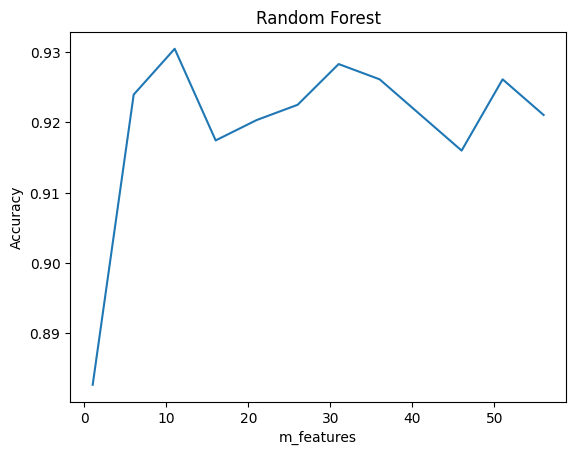
\includegraphics[width=0.8\textwidth]{images/5_b.png}
    \caption{Accuracy vs Number of features}
    \label{fig:5_b}
\end{figure}

\subsection*{Part (c)}
Plot of OOB error vs number of trees is shown in Figure \ref{fig:5_c}. Here number of feature (m) set to 11.
\begin{itemize}
    \item OOB error (0.092-0.10) is slightly higher than the test error (0.058-0.075).
    \item Both OOB error and test error are oscillating with number of trees.
\end{itemize}

\begin{figure}[h]
    \centering
    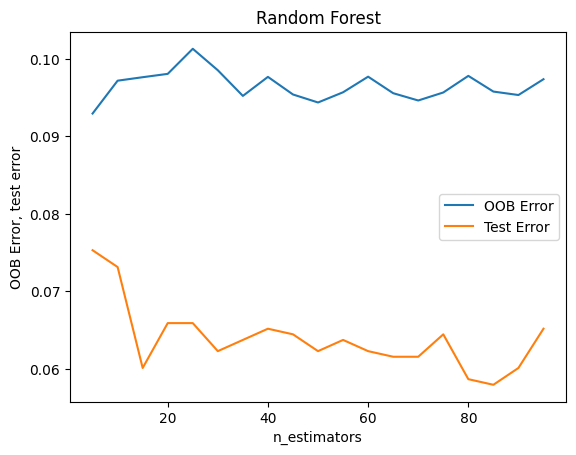
\includegraphics[width=0.8\textwidth]{images/5_c.png}
    \caption{OOB error vs Number of trees}
    \label{fig:5_c}
\end{figure}

\section*{Problem 6}
\subsection*{Part (a)}
Preprocessing steps:
\begin{itemize}
    \item Find the null value percentage in each column, and removed coulmns with null value percentage greater than 20\%.
    \item Deal with columns having data type as object:
    \begin{itemize}
        \item If column values can be directly converted to float, then convert them. Eg: int\_rate have percentage values.
        \item If unique values in column are less ($\leq$ 12) and are useful convert them to one-hot encoding. Eg: grade have values A, B, C, D, E, F, G.
        \item Else drop the column.
    \end{itemize}
    \item Modify the target loan\_status column to +1 for Fully Paid and -1 for Charged Off.
    \item Fill the null values with mean of the column.
    \item Find feature importance using Random Forest and drop columns with importance less than 0.0003. 
    \item Drop id and member\_id columns, as they are unique for each row.
\end{itemize}

\subsection*{Part (b)}
Hyperparameters tuning: \\
\textbf{Learning rate}
% table
\begin{center}
    \begin{tabular}{|c|c|c|c|}
        \hline
        Learning rate & Accuracy & Precision & Recall \\
        \hline
        0.001 & 0.84919 & 0.84919 & 1.0 \\
        0.01 & 0.97219 & 0.96829 & 1.0 \\
        0.05 & 0.98998 & 0.98834 & 1.0 \\
        0.1 & 0.99468 & 0.99385 & 0.99992 \\
        0.15 & 0.99545 & 0.99491 & 0.99975 \\
        0.2 & 0.996217 & 0.99573 & 0.99984 \\ 
        \hline
    \end{tabular}
\end{center}
\textbf{Number of trees}
% table
\begin{center}
    \begin{tabular}{|c|c|c|c|}
        \hline
        Number of trees & Accuracy & Precision & Recall \\
        \hline
        50 & 0.9951 & 0.99434 & 0.99992 \\
        100 & 0.996217 & 0.99573 & 0.99984 \\
        200 & 0.99727 & 0.99688 & 01.99992 \\
        300 & 0.99748 & 0.99712 & 0.99992 \\
        500 & 0.99769 & 0.99737 & 0.99992 \\
        700 & 0.99775 & 0.99745 & 0.99992 \\
        1000 & 0.99797 & 0.9977 & 0.99992 \\
        1250 & 0.99811 & 0.99786 & 0.99992 \\
        1500 & 0.99811 & 0.99786 & 0.99992 \\
        1700 & 0.99811 & 0.99786 & 0.99992 \\ 
        \hline
    \end{tabular}
\end{center}
Increasing the number of trees increases the accuracy, but becomes stagnant after a certain point. \\
\textbf{Max depth}
% table
\begin{center}
    \begin{tabular}{|c|c|c|c|}
        \hline
        Max depth & Accuracy & Precision & Recall \\
        \hline
        3 & 0.99811 & 0.99786 & 0.99992 \\
        5 & 0.99825 & 0.99794 & 1.0 \\
        7 & 0.99825 & 0.99794 & 1.0 \\
        9 & 0.99811 & 0.99778 & 1.0 \\
        \hline
    \end{tabular}
\end{center}
After doing hyperparameter tuning, we get:
\begin{itemize}
    \item Learning rate: 0.2
    \item Number of trees: 1250
    \item Max depth: 5
    \item Accuracy: 0.9982488091902494
    \item Precision: 0.997942048073757
    \item Recall: 1.0
\end{itemize}
\textbf{Gradient Boosting vs Decision Tree}:
\begin{itemize}
    \item Gradient Boosting:
    \begin{itemize}
        \item Accuracy: 0.9982488091902494
        \item Precision: 0.997942048073757
        \item Recall: 1.0
    \end{itemize}
    \item Decision Tree:
    \begin{itemize}
        \item Accuracy: 0.9969179041748389
        \item Precision: 0.9979388243053838
        \item Recall: 0.9984327311721521
    \end{itemize}
\end{itemize}
   
\end{document}